\section{\textit{RollBack} Solidário}

	Assim como o \textit{Time Warp}, o \textit{Rollback} Solidário é um protocolo otimista, entretanto, ele apresenta diferenças significativas na maneira com que os retornos são realizados para sincronizar os processos durante a simulação distribuída.
	
	Uma primeira diferença que pode ser citada é que no protocolo \textit{Rollback} Solidário, quando um erro de causa e efeito é identificado durante a simulação, todos os processos executam em conjunto um \textit{rollback} para um \textit{checkpoint} global consistente, enquanto no protocolo \textit{Time Warp}, em um primeiro instante, apenas o processo que identificou o erro de causa e efeito realiza o \textit{rollback}.
	
	Estas diferença na maneira de se realizar o retorno dos procesos dispensa a necessidade de se enviar anti-mensagens, que poderiam provocar \textit{rollbacks} em outros processos, evitando assim a ocorrência de \textit{rollback} em cascata.

\section{O comportamento geral do protocolo \textit{Rollback} Solidário}
	No decorrer de uma simulação, utilizando o protocolo \textit{Rollback} Solidário, assim como no \textit{Time warp}, os processos se intercomunicam através de mensagens. Porém, ao identificar um erro de causa e efeito, ou seja, ao se receber uma mensagem \textit{straggler}, o sistema se comporta da seguinte forma:

\begin{itemize}
	\item O processo que recebeu a mensagem \textit{straggler} identifica o estado salvo (\textit{checkpoint}) com tempo lógico imediatamente anterior ao \textit{timestamp} da mensagem.
	\item O sistema se encarrega de selecionar o \textit{checkpoint} global consistente que contenha este estado identificado e que cause a menor sobrecarga durante o  \textit{rollback} (mínimo possível de eventos para se retornar).
	\item Toda a simulação realiza o retorno à este \textit{checkpoint} global consistente de maneira uniforme.
\end{itemize}

\section{Recuperação dos Estados Durante um \textit{Rollback}}
A eficiência do protocolo \textit{Rollback} Solidário está diretamente ligada em como ele retorna à um \textit{checkpoint} global consistente após identificar uma inconsistência na simulação. O \textit{checkpoint} global consistente a ser selecionado deve gerar o menor custo para o sistema. Para isto, deve-se garantir que os processos voltem a menor distância possível necessária para recompôr o processamento.

	Considerando o exemplo da figura~\ref{fig:linhasrec}, sabe-se que em relação a seus tempos lógicos  tem-se $t''<b'<t'<t$. Assim sendo, supondo que o processo $p_{1}$ receba uma mensagem no tempo $t$, gerando um evento que deveria ter sido executada no tempo $t'$, ocorre que neste momento o sistema deve retornar ao último \textit{checkpoint} global consistente que contenha o processo $b'$, que neste caso é o corte B. Porém, supondo que o processo $P_1$ recebe, no tempo $t$, uma mensagem que gera um evento a ser processado no tempo $t''$, anterior ao evento $b'$ , não pode-se admitir o corte B como linha de recuperação, devido ao tempo lógico de $b'$ ser maior que o tempo lógico de $t''$. Acontece aí então um \textit{rollback} para a linha de recuperação A. 
	
	Nota-se, nessa situação, que nem todos os processos precisam voltar para a mesma linha de recuperação. No exemplo da figura~\ref{fig:linhasrec}, tanto os processos P2 e P3 podem permanecer com os mesmos \textit{checkpoints} do corte B, uma vez que não houve troca de mensagens por parte dos processos entre os cortes A e B.
	
	Para garantir a eficiência do protocolo, deve-se garantir que a linha de recuperação preserve ao máximo os eventos já processados. Para isso, é necessário armazenar várias linhas de recuperação que passem por um mesmo \textit{checkpoint}.

\begin{figure}[htb]
  \centerline{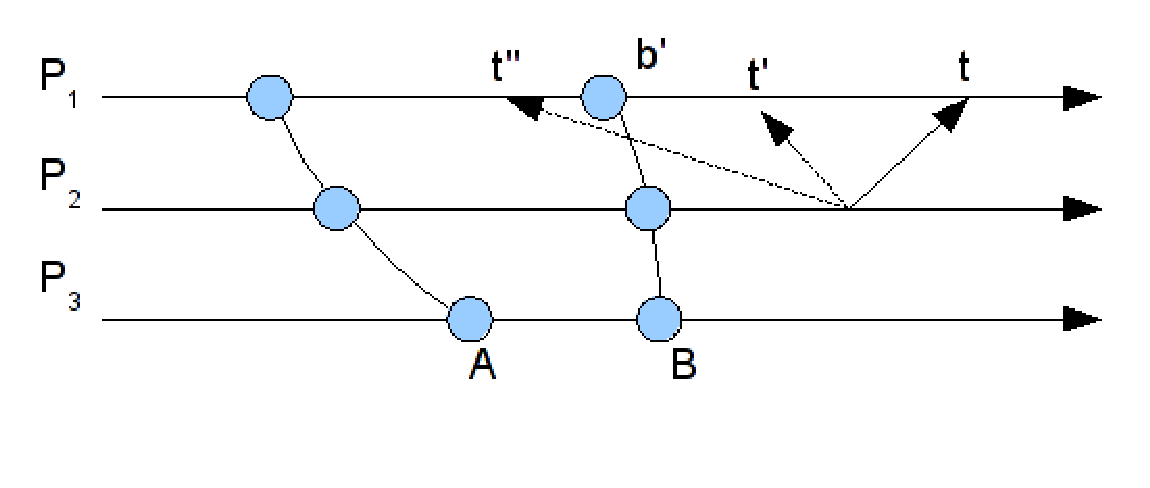
\includegraphics[scale=0.6]{cortes_rollback.eps}}
  \caption{Linhas de recuperação.}
\label{fig:linhasrec}
\end{figure}	


\section{Uma abordagem utilizando \textit{checkpoints} síncronos}
	Mecanismos de \textit{checkpoints} síncronos são mecanismos que exigem que os processos realizem seus checkpoints em conjunto para a obtenção de um \textit{checkpoint} global consistentes.	 Para o protocolo \textit{Rollback} Solidário utilizando \textit{checkpoints} síncronos são apresentadas as extenções dos os algorítimos \textit{Sync-and-Stop}\cite{Plank93}  e \textit{Chandy-Lamport}\cite{ChandyLamport}.


\section{Rollback Solidário utilizando mecanismos de \textit{checkpoints} Semi-Síncronos}

	Para a construção da linha de recuperação na abordagem semi-síncrona, um processo, denominado processo observador, fica encarregado de receber os vetores de dependência associados aos respectivos \textit{checkpoints} de cada processo e identificar o \textit{checkpoint} global consistente para onde a simulação deve retornar.

	Ao realizar um \textit{checkpoint}, um processo envia ao observador um vetor com as suas dependências. Com isto, o processo observador constrói um matriz quadrada $M$ de ordem $n$, onde $n$ é o número de processos da simulação. Cada linha $i$ da matriz é o vetor de dependência de um processo $p_i$, que contém as informações de dependência do último \textit{checkpoint} realizado por esse processo $p_i$. 

	A matriz é iniciada com o primeiro \textit{checkpoint} de cada processo. Como todos os processos no início da simulação estão num mesmo evento inicial, a matriz $M$ é iniciada como uma matriz identidade.

	A diagonal principal da matriz $M$ poderá indicar uma linha de recuperação da simulação. Para que esta linha de recuperação seja válida, todos os elementos de uma coluna que não fizerem parte da diagonal principal da matriz devem possuir valores menores do que o elemento pertencente à diagonal.  

	Para garantir que todas as possíveis linhas de recuperação sejam identificados um novo vetor de dependência é recebido pelo processo observador, o último vetor referente ao processo que realizou o \textit{checkpoint} não deve ser descartado, mas sim armazenado para futuras consultas.

	A solução para se armazenar os diversos vetores está em utilizar, ao invés de matriz quadrada uma lista encadeada para cada processo, cada uma contendo os vetores de dependência.

	Ao receber um aviso de \textit{rollback}, proveniente de algum processo, cabe ao processo observador percorrer as listas e identificar os \textit{checkpoints} adequados para constituir a linha de recuperação correspondente.
	
	